\documentclass[tikz,border=8pt]{standalone}
% Shared look for every TikZ diagram. Load with \input{../../tools/tikz-style.tex}
\usepackage[T1]{fontenc}
\usepackage{lmodern}
\renewcommand{\sfdefault}{lmr}  % diagrams use the same serif as the text
\usetikzlibrary{arrows.meta, positioning, shapes.geometric, calc, fit, backgrounds}
\definecolor{cblue}{HTML}{4C78A8}
\definecolor{corange}{HTML}{F58518}
\definecolor{cgreen}{HTML}{54A24B}
\definecolor{cred}{HTML}{E45756}
\definecolor{cpurple}{HTML}{B279A2}
\definecolor{cgrey}{HTML}{6B6B6B}
\tikzset{
  every picture/.style={font=\sffamily, line width=1.2pt},
  box/.style={draw=#1, fill=#1!12, rounded corners=4pt, align=center, inner sep=7pt, minimum height=1.1cm},
  box/.default=cgrey,
  arrow/.style={-{Stealth[length=3mm]}, draw=cgrey, line width=1.4pt},
  title/.style={font=\sffamily\bfseries\Large},
  note/.style={font=\sffamily\small, text=cgrey, align=center},
}
\AtBeginDocument{\hyphenpenalty=10000 \exhyphenpenalty=10000}

\begin{document}
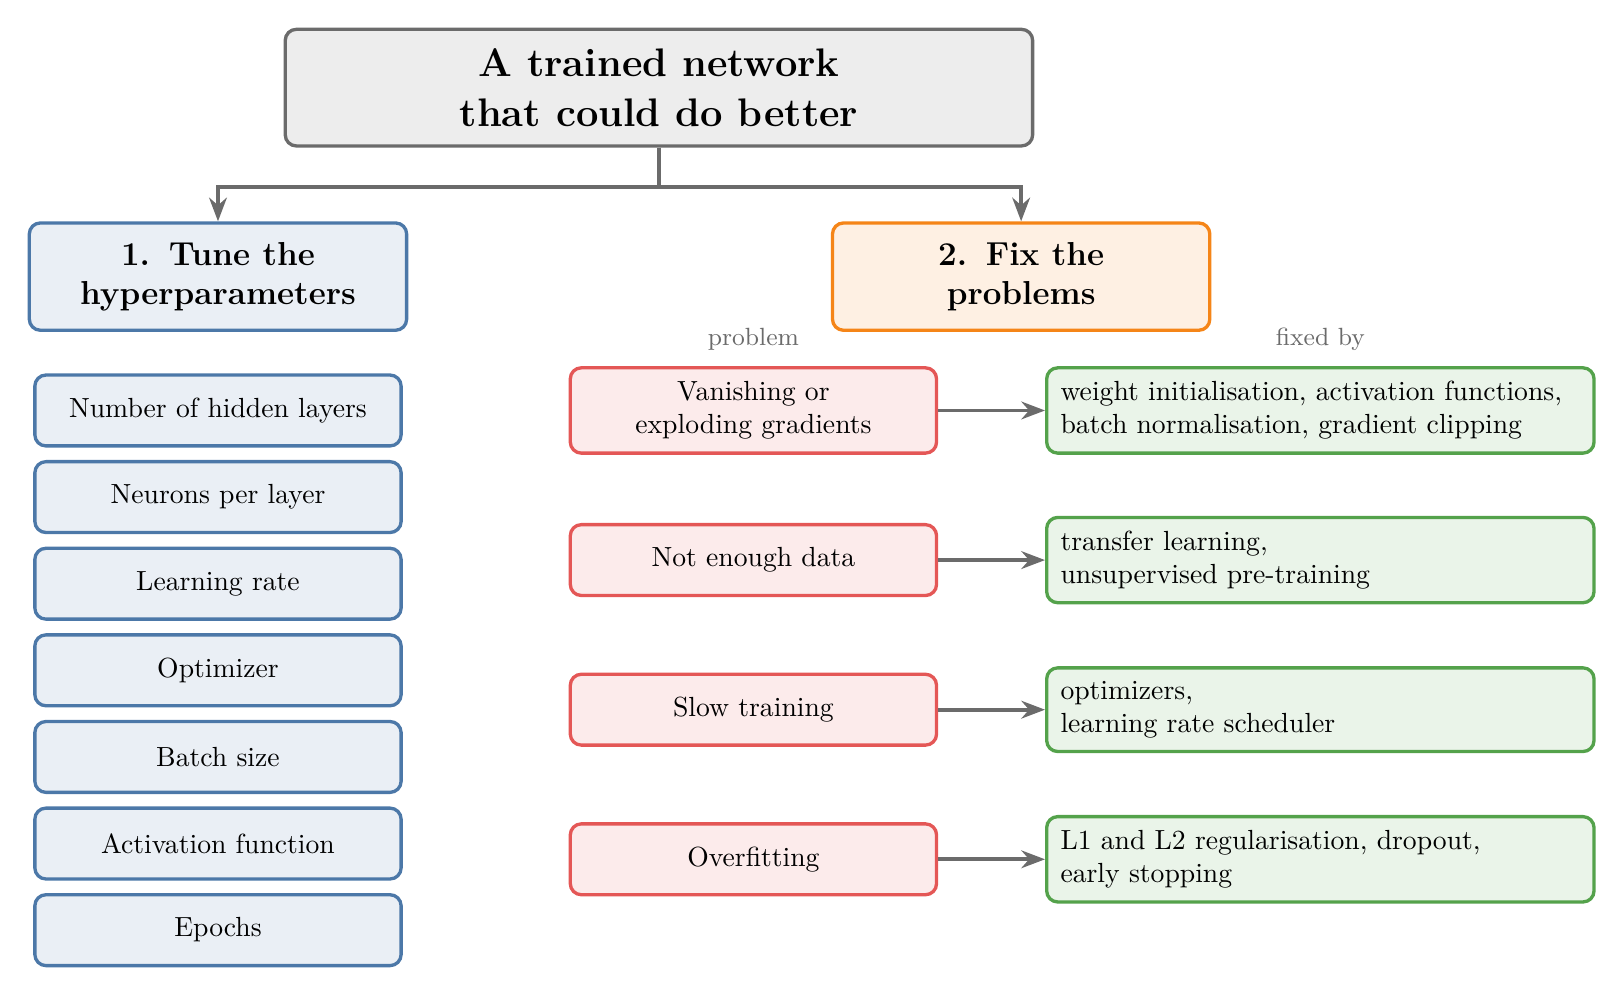
\begin{tikzpicture}[
  item/.style={box=#1, text width=4.3cm, minimum height=0.9cm, inner sep=5pt},
  fix/.style={box=#1, text width=6.6cm, minimum height=0.9cm, inner sep=5pt, align=left},
  head/.style={box=#1, text width=4.3cm, font=\sffamily\bfseries\large}]
  % root
  \node[box=cgrey, font=\sffamily\bfseries\Large, text width=9cm] (root) at (0, 0) {A trained network that could do better};
  % branch 1: hyperparameters
  \node[head=cblue] (hp) at (-5.6, -2.4) {1. Tune the\\hyperparameters};
  \foreach \t [count=\i] in {Number of hidden layers, Neurons per layer, Learning rate, Optimizer, Batch size,
                             Activation function, Epochs} {
    \node[item=cblue] (h\i) at (-5.6, -3.0 - 1.1*\i) {\t};
  }
  % branch 2: problems -> fixes
  \node[head=corange] (pr) at (4.6, -2.4) {2. Fix the\\problems};
  \node[note] at (1.2, -3.2) {problem}; \node[note] at (8.4, -3.2) {fixed by};
  \node[item=cred]    (p1) at (1.2, -4.1) {Vanishing or\\exploding gradients};
  \node[item=cred]    (p2) at (1.2, -6.0) {Not enough data};
  \node[item=cred]    (p3) at (1.2, -7.9) {Slow training};
  \node[item=cred]    (p4) at (1.2, -9.8) {Overfitting};
  \node[fix=cgreen]   (f1) at (8.4, -4.1) {weight initialisation, activation functions,\\batch normalisation, gradient clipping};
  \node[fix=cgreen]   (f2) at (8.4, -6.0) {transfer learning,\\unsupervised pre-training};
  \node[fix=cgreen]   (f3) at (8.4, -7.9) {optimizers,\\learning rate scheduler};
  \node[fix=cgreen]   (f4) at (8.4, -9.8) {L1 and L2 regularisation, dropout,\\early stopping};
  \draw[arrow] (root.south) -- ++(0,-0.5) -| (hp.north);
  \draw[arrow] (root.south) -- ++(0,-0.5) -| (pr.north);
  \foreach \i in {1,...,4} {
    \draw[arrow] (p\i.east) -- (f\i.west);
  }
\end{tikzpicture}
\end{document}
